\section{Sistema de Gerência de Memória}
\label{sec:memoria}

Embora não seja exatamente um requerimento da \acs{R7RS}-small, esta implementação
possui também um mecanismo de gerência de memória automatizado, o que definiu
em diversas formas as escolhas utilizadas para representação dos valores em
tempo de execução nesta implementação. Historicamente Lisp está tão
intimamente ligada à gerência automatica de memória, visto que foi a primeira
linguagem de programação a utilizar a técnica[20], que a escolha por incluir um
mecanismo de gerência automática de memória se deu pelo interesse em descrever
o mesmo algoritmo utilizado por McCarthy em sua implementação original.

Os objetos descritos na linguagem \textit{Scheme} podem ser divididos em dois
tipos de valores, em relação a necessitarem ou não de alocação de memória
dinâmica. Entre os valores que não necessitam de alocação de memória dinâmica,
chamados daqui em diante de valores imediatos, encontram-se os inteiros,
booleanos, caracteres e alguns valores especiais como o marcador de lista
vazia. Estes, são implementados na forma de ``ponteiros etiquetados''
(\textit{tagged pointers}), em que os dados ocupam os 62 bits mais
significativos de uma palavra de 64 bits, e os 2 bits menos significativos são
utilizados para identificar os valores como imediatos, identificação preliminar
do tipo e diferenciar estes valores dos demais ponteiros no sistema.

Os demais, como funções, strings, pares e quaisquer estruturas de dados
complexas, são implementados seguindo uma estrutura de dados comum a todos, de
forma a simplificar a implementação do mecanismo de gerência de memória.
Nestes, os 2 bits menos significativos têm obrigatóriamente o valor zero,
criando a necessidade de um alinhamento de 4 bytes para cada objeto alocado em
memória. A estrutura utilizada para estes valores complexos é a descrita a
seguir e pode ser vista na figura \ref{fig:celula}:

Uma palavra de 64 bits é utilizada para manter informações de tipo, dados
relacionados à gerência de memória e se o objeto armazenado pode ser
modificado. Entre estes, deve-se ressaltar os dados de gerência de memória que
indicam:

\begin{itemize}

\item se o objeto foi visitado pelo sistema de gerência de memória durante a
coleta (\sctt{gc\_has\_mark});

\item  se o objeto está em uso pelo sistema (\sctt{gc\_is\_in\_use});

\item  se o mecanismo de gerência de memória deve analisar seu filho esquerdo
(\sctt{mark\_policy\_first}) e/ou seu filho direito
(\sctt{mark\_policy\_second});

\item  ou se a memória para este objeto nunca deve ser liberada
(\sctt{gc\_always\_marked}).

\end{itemize}

Além destas informações, um conjunto de bits é utilizado para manter a
informação sobre o tipo destes objetos, para questões de despacho de funções e
checagem de tipos. Oito bits foram utilizados para este fim, embora devido ao
grande espaço não utilizado na estrutura mais possam ser utilizados para
estender o mecanismo de tipos caso seja necessário.

Em seguida, duas outras palavras de 64 bits são utilizadas para armazenar as
demais partes da estrutura de dados. Estas duas palavras (chamados daqui em diante
simplesmente de  \textit{slots}) armazenam valores arbitrários do sistema, usando a mesma técnica
de tagged pointers mencionada anteriormente, em que valores imediatos são
armazenados diretamente e valores complexos são armazenados como ponteiros para
outras estruturas idênticas às aqui descritas. 

Esta estrutura simples representa diretamente a estrutura de dados mais
utilizada em um dialeto Lisp: a ``célula cons'' que é utilizada para, entre
outras coisas, representar listas, como a representação interna do código
fonte. Uma célula cons nada mais é que um par de dois outros valores quaisquer
da linguagem. Esta estrutura é utilizada para todos os demais valores que não
podem ser representados como valores imediatos, o que é bom o suficiente já que
o objetivo desta implementação não é o de otimizar para espaço ou tempo.

\begin{figure}[h!]
\centering
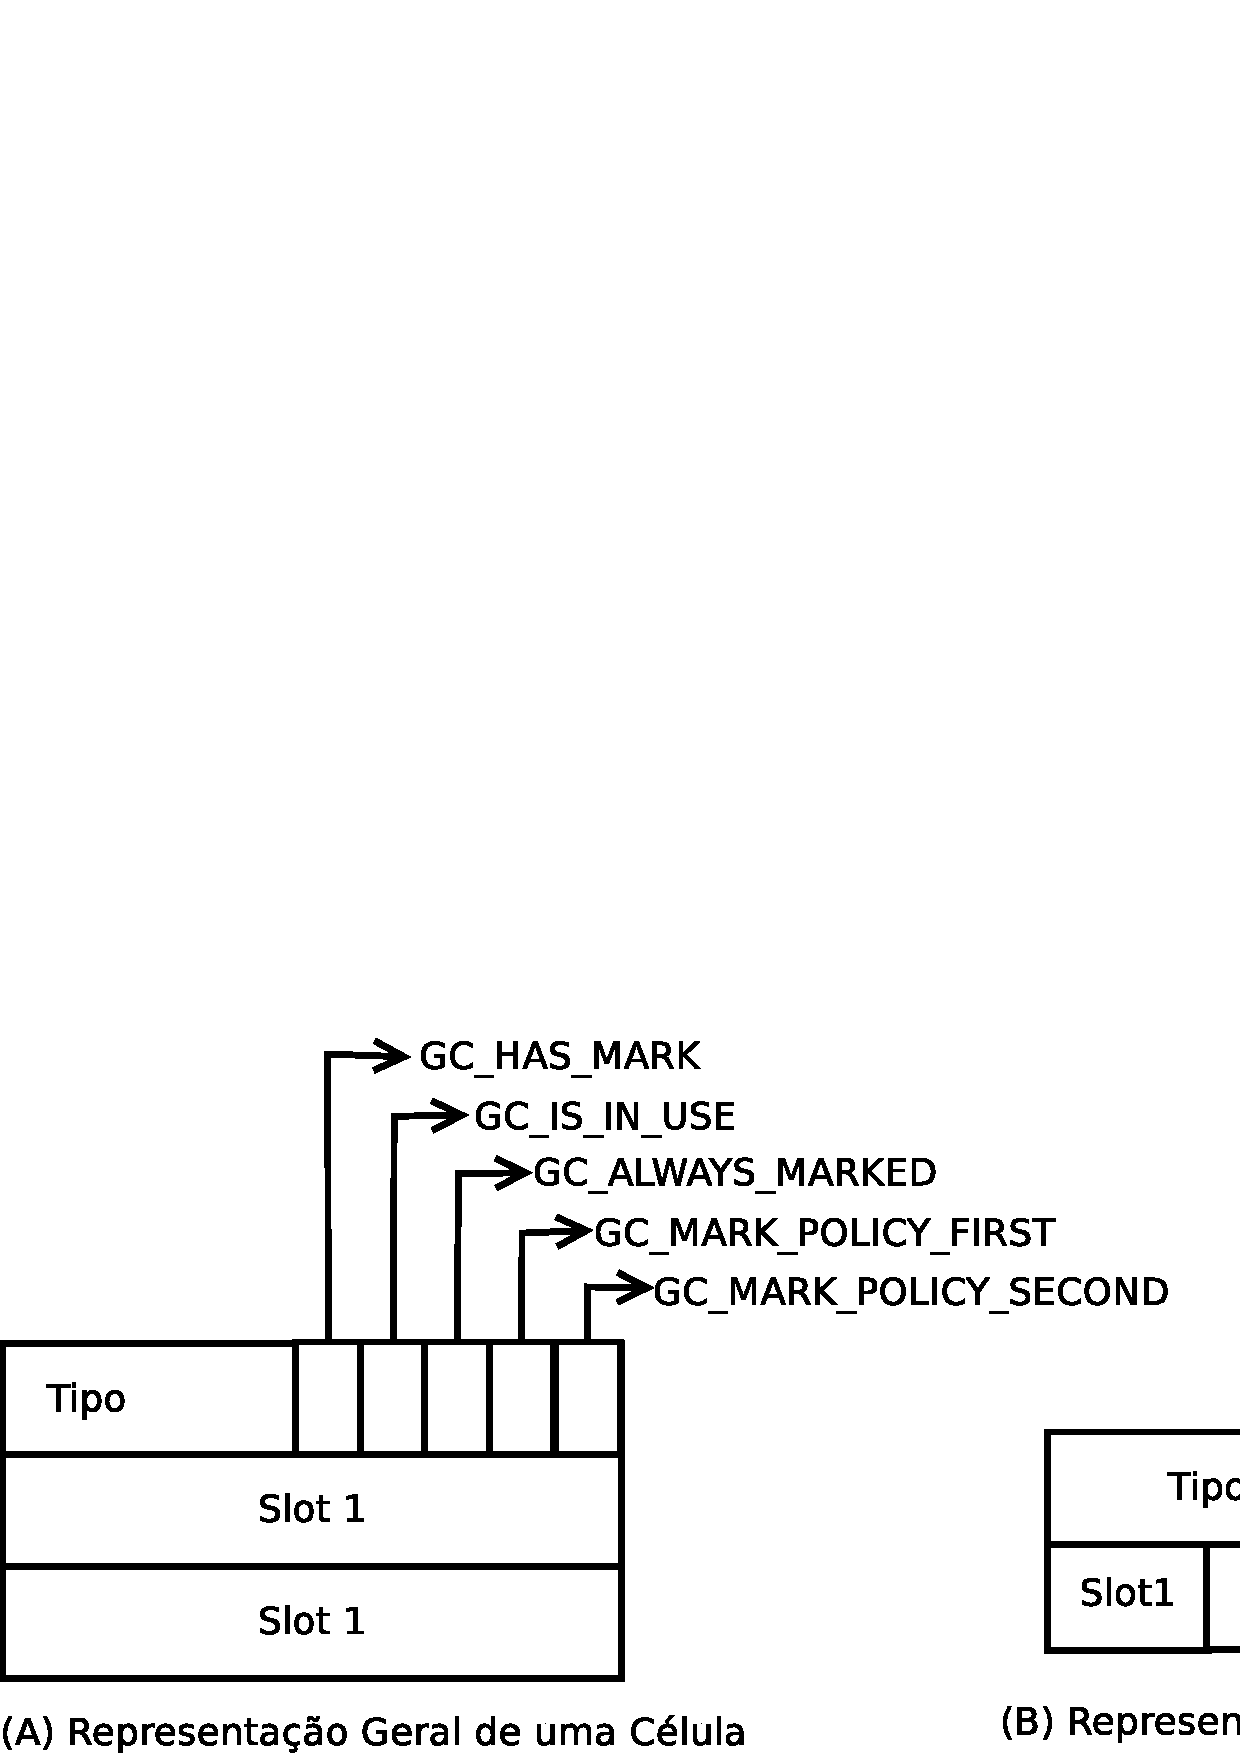
\includegraphics[width=0.9\textwidth]{../images/celula.pdf}
\caption{Duas visões para a estrutura de célula de memória utilizada}
\label{fig:celula}
\end{figure}

Como todos os valores não imediatos são representados utilizando esta
estrutura de armazenamento duplo em \textit{slots}, em alguns casos apenas um dos \textit{slots}
de armazenamento é utilizado, em outros casos ambos. Na figura \ref{fig:memoria}
pode-se verificar alguns exemplos de como a memória é estruturada quando
representa alguns objetos.

\begin{figure}[h!]
\centering
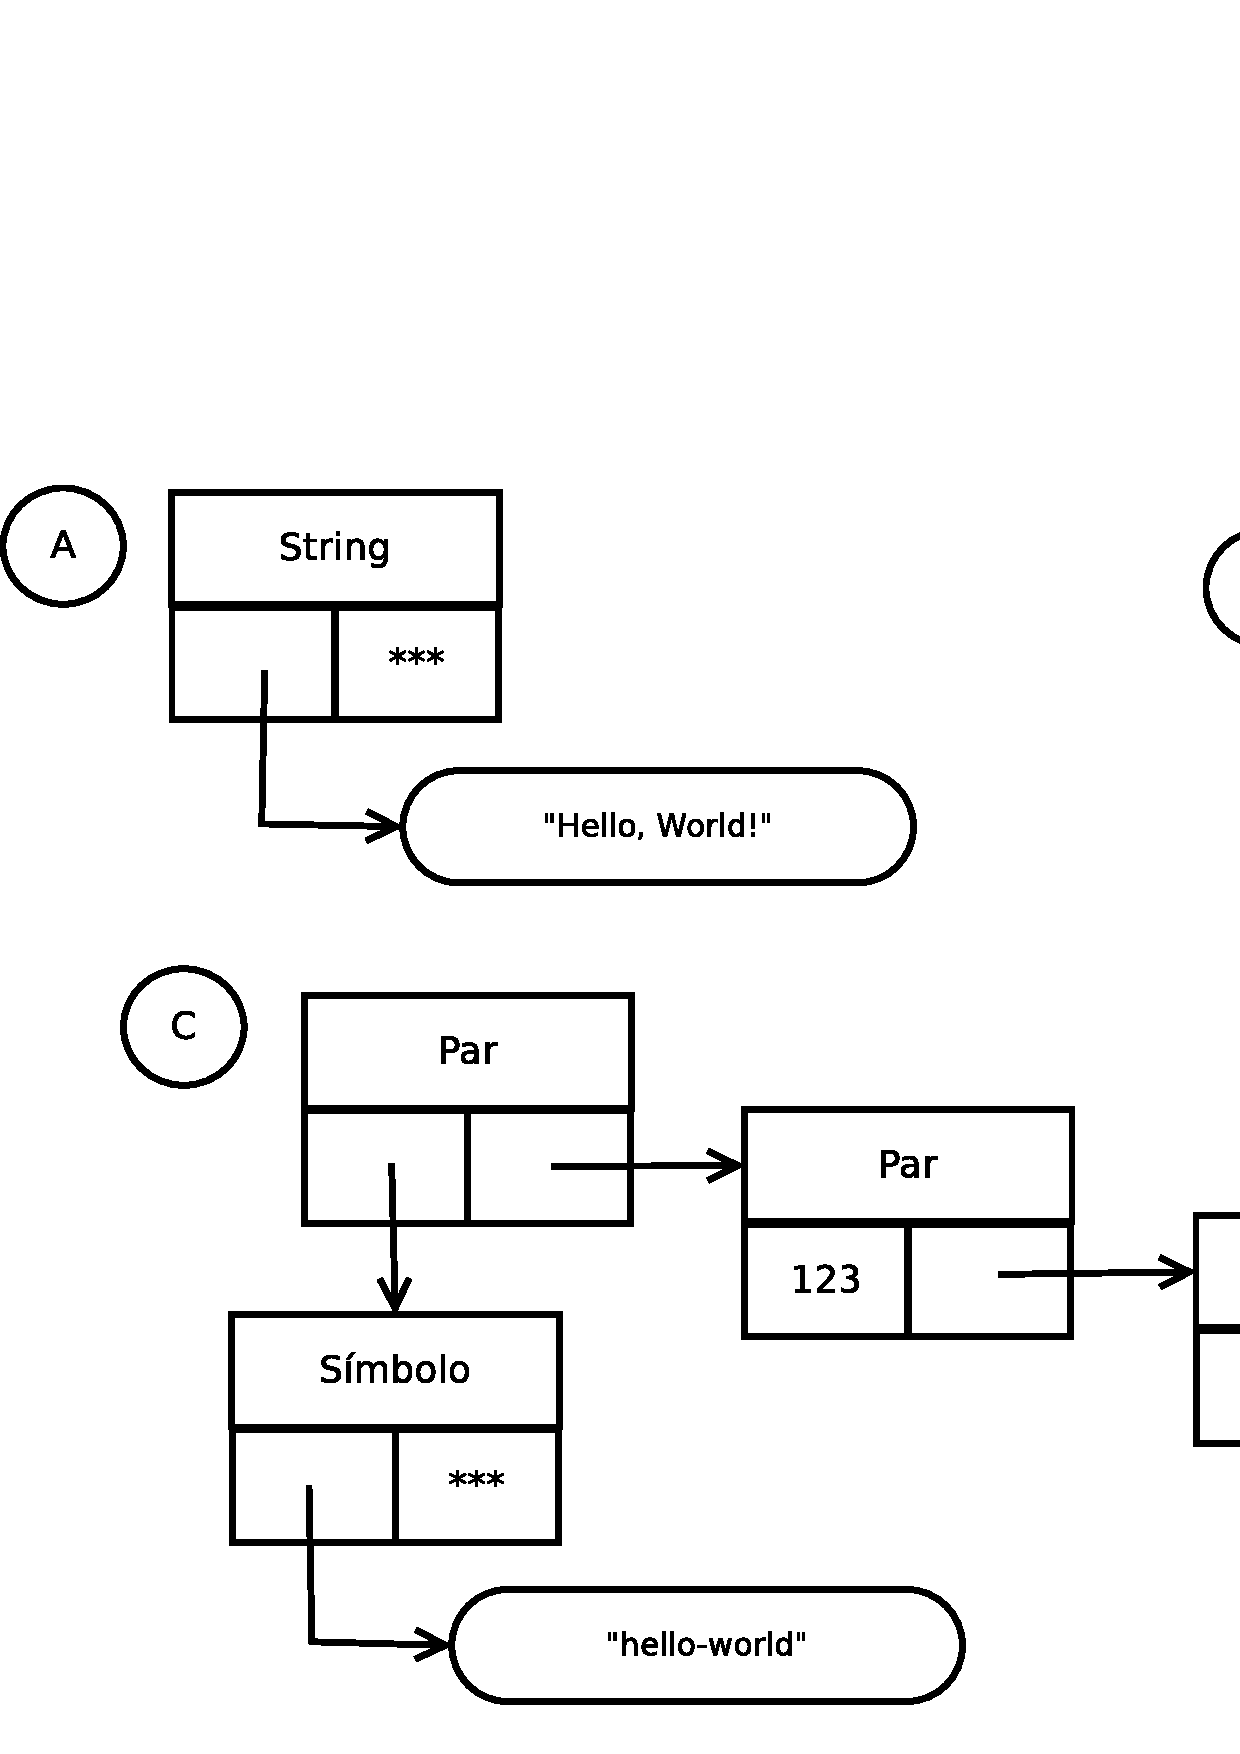
\includegraphics[width=1\textwidth]{../images/memoria.pdf}
\caption{Estrutura de objetos em memória. (A) uma string; (B) uma função
         primitiva; (C) uma lista com um símbolo e alguns valores imediatos.}
\label{fig:memoria}
\end{figure}

Dado que todos os valores armazenados por meio de alocações dinâmicas possuem o
mesmo formato e é trivialmente possível identificar ponteiros para outros
objetos na estrutura utilizada, fica simples implementar um mecanismo de
gerência de memória. O algoritmo utilizado é o mesmo descrito por John McCarthy
em sua implementação original de Lisp[20], e consiste dos seguintes passos:

\begin{itemize}

\item Inicialize a memória como um bloco de elementos livres, prontos a serem
utilizados;
 
\item Configure este bloco de forma que o segundo \textit{slot} de cada elemento aponte
para o próximo, formando uma lista encadeada de elementos livres;
 
\item A cada nova alocação necessária, obtenha um elemento da lista de
elementos livres;
 
\item Quando não houver mais elementos livres, identifique os elementos que
estão em uso e marque-os (fase de marcação);
 
\item Após marcar os elementos em uso, varra a área de memória utilizada
retornando todos os elementos que não estão sendo utilizados para a lista de
elementos livres (fase de varredura).

\end{itemize}

Para identificar os elementos que estão em uso, basta seguir as cadeias de
referências dos \textit{slots} da estrutura descrita acima, a partir de cada um
dos registradores da máquina virtual, uma estrutura auxiliar, chamada pilha de
proteção de memória, que é usada para manter referências para termos
intermediários de uma computação para evitar que uma coleta remova objetos
úteis antes destes serem postos em uso, e uma outra estrutura utilizada pelo 
sistema de macros que guarda referência para cada um dos blocos de código
relacionados a uma macro no sistema. Cada elemento encontrado nestas cadeias
é então marcado como sendo utilizado.

Dado que os elementos são alocados dentro de um ou mais blocos conhecidos de
memória, é fácil iterar por todos os elementos alocados, reinserindo-os na
lista de elementos livres se não estiverem marcados e desmarcando os que
estiverem, para deixar o estado geral da memória pronto para outro ciclo de
coleta.

Por questões de otimização uma flag (\sctt{gc\_always\_marked}) indica objetos
que não são varridos por gerenciarem a própria memória e nunca serem
desalocados após serem criados. E por haver valores que não ocupam ambos os
\textit{slots}, ou ainda por haver valores que guardam dados que não são controlados
pela gerência de memória nestes \textit{slots}, algumas flags
(\sctt{mark\_policy\_first}, \sctt{mark\_policy\_second}) controlam se é
necessário continuar o percurso por cada um dos \textit{slots} de um elemento.

Este modelo simples de gerência de memória, conhecido como Mark \& Sweep pelas
duas fases utilizadas[17], é suficiente para garantir que a máquina virtual
utilize plenamente a memória disponível antes de terminar por falta de
memória.

